\lab{Applications}{Least-squares fitting I}{Least-squares fitting I}
\label{LeastSquaresCircle}

\objective{This section will introduce Least Squares and teach a more advanced application of Least Squares: fitting data to an circle.}
\section*{Least Squares}

It is well known that the displacement of a spring is proportional to the force acting upon it, that is, $F = k x$.  The proportionality constant $k$ is called Hooke's spring constant.  Consider a laboratory experiment where different loads are placed on a spring and the displacement is measured and recorded in the table below:
\vspace{5mm}\\
\begin{center}
\begin{tabular}{|c|c|}
	\hline
x & F \\
(cm) & (dyne)\\
\hline
1.04  & 3.11 \\
2.03  &  6.01\\
2.95  &  9.07\\
3.92  &  11.99\\
5.06  &  15.02\\
6.00  &  17.91\\
7.07  &  21.12\\
\hline
\end{tabular}
\end{center}
\vspace{5mm}
To find the spring constant $k$, we simply need to solve the following linear system
\[
\begin{pmatrix}
1.04\\
2.03\\
2.95\\
3.92\\
5.06\\
6.00\\
7.07\\
\end{pmatrix}
\begin{pmatrix}k\end{pmatrix} = 
\begin{pmatrix}
3.11 \\
6.01\\
9.07\\
11.99\\
15.02\\
17.91\\
21.12\\
\end{pmatrix}.
\]
However, there is no solution to this system because it is overdetermined.  Instead, we seek the ``best'' $k$ that fits the data.  Least squares (which we mentioned in a previous exercise) allows us to find that ``best'' solution. We can find the least squares solution by computing the following in Python:
\begin{lstlisting}[style=python]
: A = sp.vstack([1.04,2.03,2.95,3.92,5.06,6.00,7.07])
: b = sp.vstack([3.11,6.01,9.07,11.99,15.02,17.91,21.12])
: k = sp.dot(sp.dot(la.inv(sp.dot(A.T,A)),A.T),b);k
: # Using the built in least squares function this is just: k=la.lstsq(A,b);k
array([[ 2.99568294]])
\end{lstlisting}
Hence, we find the spring constant to be $k = 2.9957$.  We plot the data against the best fit as follows:
\begin{figure}[h!]
\label{fig1}
\begin{center}
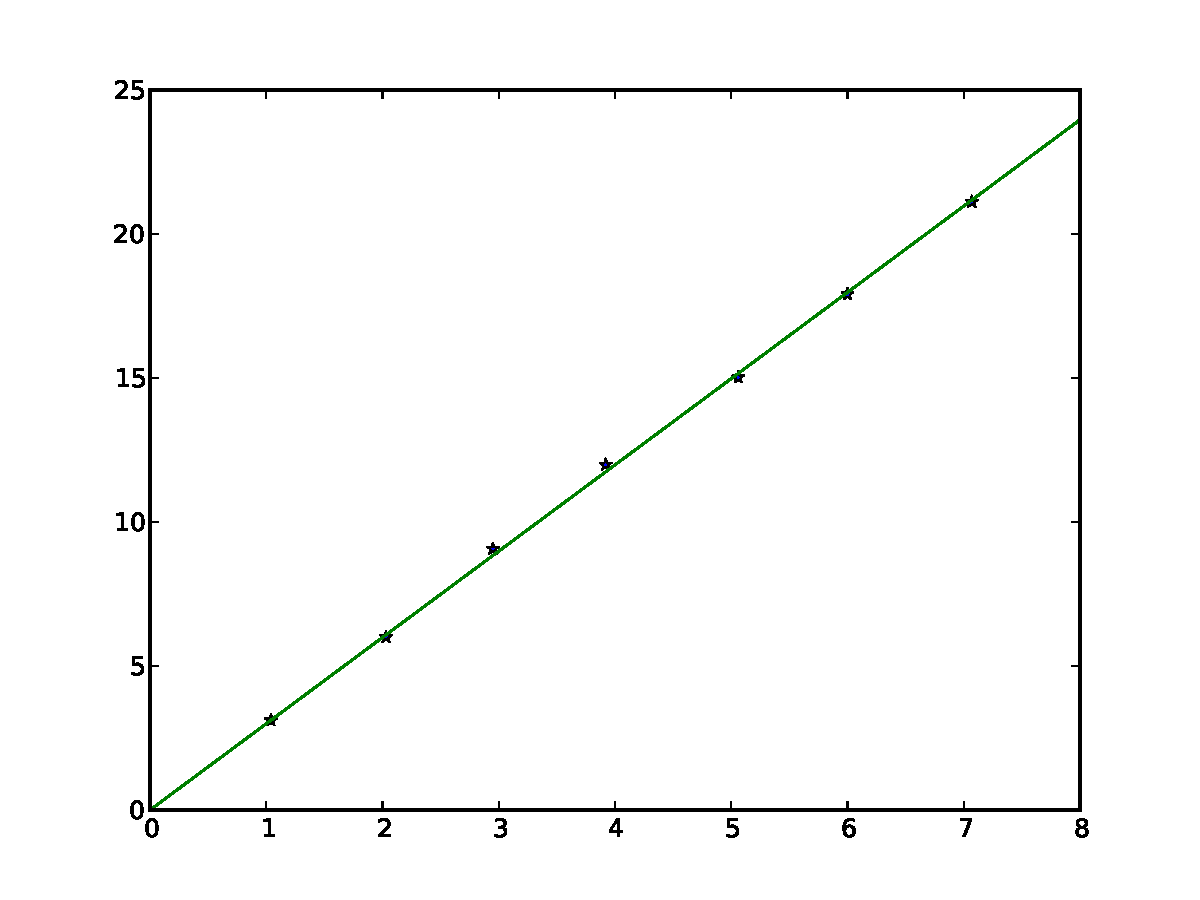
\includegraphics[scale = .6]{lab9_line_py}
\caption{The graph of the spring data together with its linear fit}
\label{Fig:SpringFit}
\end{center}
\end{figure}

\begin{lstlisting}[style=python]
: x0 = sp.linspace(0,8,100)
: y0 = k[0]*x0
: from matplotlib import pyplot as plt
: plt.plot(A,b,'*',x0,y0)
: plt.show()
\end{lstlisting}
See Figure \ref{Fig:SpringFit} to see how well the line fits the data.


\section*{General Line Fitting}

Suppose that we wish to fit a general line, that is $y=m x+b$, to the data set $\{(x_k,y_k)\}^n_{k=1}$.  Assume that the line does not cross through the origin, as in the previous example.  Then we seek both a slope and a $y$-intercept.  In this case, we set up the following linear system $A x = b$, or more precisely
\[
\begin{pmatrix}
x_1 & 1\\
x_2 & 1\\
x_3 & 1\\
\vdots & \vdots\\
x_n & 1
\end{pmatrix}
\begin{pmatrix}
m\\
b
\end{pmatrix}=
\begin{pmatrix}
y_1\\
y_2\\
y_3\\
\vdots\\
y_n
\end{pmatrix}.
\]
Note that $A$ has rank $2$ as long as not all of the $x_k$ values are the same.  Hence, the least squares solution will fit the best line for this data.


\begin{problem}
Download the file lab9.txt from the following link:
\url{http://www.math.byu.edu/~jeffh/teaching/m343h/lab9.txt}
You can load this datafile by typing
\li{lab9 = sp.genfromtxt("lab9.txt")}
Now the data is available in the array \li{lab9}.
This consists of two columns corresponding to the $x$ and $y$ values of a given data set.  Use least squares to find the slope and $y$-intercept that best fits the data.  Then plot the data points and the line on the same graph.  Finish off the problem with a discussion of what you've learned.
\end{problem}

\section*{Fitting data to a circle}

Recall that the equation of a circle, with radius $r$ centered at $(c_1,c_2)$, is given by
\begin{equation}
\label{circle}
(x-c_1)^2 + (y-c_2)^2 = r^2.
\end{equation}
Suppose we are given a set of data points closely forming a circle $\{(x_i,y_i)\}^n_{i=1}$.  The ``best'' fit is found via least squares by expanding \eqref{circle} to get
\[
2 c_1 x + 2 c_2 y + c_3 = x^2 + y^2,
\]
where $c_3 = r^2 - c_1^2 - c_2^2$.  Then we can write the linear system $A x = b$ as
\[
\begin{pmatrix}
2 x_1 & 2 y_1 & 1\\
2 x_2 & 2 y_2 & 1\\
\vdots & \vdots & \vdots \\
2 x_n & 2 y_n & 1
\end{pmatrix}
\begin{pmatrix}
c_1\\
c_2\\
c_3
\end{pmatrix}=
\begin{pmatrix}
x_1^2 + y_1^2\\
x_2^2 + y_2^2\\
\vdots\\
x_n^2 + y_n^2
\end{pmatrix},
\]
where the matrix $A$ and the vector $b$ are obtained by the given data and the unknown $x$ contains the information about the center and radius of the circle and is obtained by finding the least squares solution.

\section*{Example}

In this section, we fit the following points to a circle:
\begin{align*}
&(134,76),(104,146),(34,176),(-36,146),\\
&(-66,76),(-36,5),(34,-24),(104,5),(134,76)
\end{align*}

We enter them into Python as a $9\times 2$ array:
\begin{lstlisting}[style=python]
: P = sp.array([[134,76],[ 104,146],[ 34,176],[ -36,146],[ -66,76],[ -36,5],[ 34,-24],[ 104,5],[ 134,76]])
\end{lstlisting}
Then we can separate the $x$ and $y$ coordinates by the commands \li{P[:,0]} and \li{P[:,1]}, respectively.  Hence, we compute $A$ and $b$ by entering the following:
\begin{lstlisting}[style=python]
: A = sp.column_stack((2*P,sp.ones((9,1),dtype=sp.int_)))
: b = P[:,0]**2 + P[:,1]**2
\end{lstlisting}
Hence, we get the least squares solution
\begin{lstlisting}[style=python]
: x = sp.dot(sp.dot(la.inv(sp.dot(A.T,A)),A.T),b)
\end{lstlisting}
Then we find $c_1$, $c_2$, and $r$ by:
\begin{lstlisting}[style=python]
: c1 = x[0]
: c2 = x[1]
: c3 = x[2]
: r = sp.sqrt(c1**2 + c2**2 + c3)
\end{lstlisting}
We plot this by executing
\begin{lstlisting}[style=python]
: theta = sp.linspace(0,2*sp.pi,200)
: plt.plot(r*sp.cos(theta)+c1,r*sp.sin(theta)+c2,'-',P[:,0],P[:,1],'*')
: plt.show()
\end{lstlisting}


\begin{problem}
Download the file lab10.txt from the following link:
\url{http://www.math.byu.edu/~jeffh/teaching/m343h/lab10.txt}
You can load this datafile into Python by typing
\begin{lstlisting}[style=python]
: lab10 = sp.genfromtxt("lab10.txt")
\end{lstlisting}
Now the data is available in the matrix \li{lab10}.  This consists of two columns corresponding to the $x$ and $y$ values of a given data set.  Use least squares to find the center and radius of the circle that best fits the data.  Then plot the data points and the circle on the same graph.  Finish off the problem with a discussion of what you've learned.
\end{problem}

\begin{problem}
The general equation for an ellipse is:
\[
A(x-x_0)^2 + B(x-x_0)(y-y_0) + C(y-y_0)^2 = 1
\]

Write a program that uses least squares to fit data to an ellipse. One option to finding the center point $(x_0,y_0)$ is to use the mean function. Test the program on \li{lab10}. Also test it against sp.dot(lab10,sp.array([[2,0],[0,1]]) ) . Plot the result. How well does your function work?
\end{problem}
